%!TEX TS-program = xelatex
%!TEX encoding = UTF-8 Unicode
\documentclass[12pt, parindent=0]{article} % use larger type; default would be 10pt

%----------------------------------------------------------------------------------------
%   PACKAGES
%----------------------------------------------------------------------------------------
\usepackage{tablefootnote}
\usepackage{amsmath,amsfonts,amsthm} % Math packages
\usepackage{mathtools}
\usepackage{lipsum} % Used for inserting dummy 'Lorem ipsum' text into the template
\usepackage{datetime}
\usepackage{xfrac}
\usepackage{changepage} % for adjusting the width
\usepackage{gensymb}
\usepackage{subcaption}
\usepackage{sectsty}
\usepackage{xcolor}
\usepackage{verbatim}
\usepackage{titlesec}
\usepackage{color}
\usepackage{fixltx2e} %helps the [H] problem! 10/2/2015
\usepackage{float} % Not have your figures fly around  - use [H]
\usepackage{booktabs} % for much better looking tables
\usepackage{array} % for better arrays (e.g matrices) in maths
\usepackage{paralist} % very flexible & customisable lists (eg. enumerate/itemize, etc.)
\usepackage{verbatim} % adds environment for commenting out blocks of text & for better verbatim
\usepackage{subfig} % make it possible to include more than one captioned figure/table in a single float
\usepackage[export]{adjustbox}
\usepackage{pdfpages} % For pdf inputs
\usepackage{import} % for subfolder inputs
\usepackage{metalogo} % for the fucking logo
\usepackage{listings}
\usepackage{mdwlist} % for tight lists
\usepackage{csquotes} % provide the \enquote command for quick quotes
%\usepackage{import} % for subfolder inputs
\usepackage{letltxmacro} % better roots
\usepackage{xspace} % for correct spacing
\usepackage{multicol} % for the multicol environment
%\usepackage{hyperref}
\usepackage{sidecap} % for sided captions
\usepackage{wrapfig}

% enable system font access
\usepackage{fontspec}
%----------------------------------------------------------------------------------------
%   FONT CONFIGURATIONS
%----------------------------------------------------------------------------------------

\setmainfont{Palatino Linotype}
\newfontfamily{\maintext}{Palatino Linotype}
\newfontfamily{\stressed}{Helvetica}
%\newfontfamily\secfont{Arial}
%\newfontfamily{\exotic}{Arial}
%\newfontfamily{\math}{Arial}
\setsansfont{Arial}

%----------------------------------------------------------------------------------------
%   DOCUMENT CONFIGURATIONS
%----------------------------------------------------------------------------------------
\definecolor{MediumBlue}{rgb}{0 ,0 ,205}
\definecolor{Blue}{rgb}{0 ,0 ,255}
\definecolor{RoyalBlue}{rgb}{65,105,225}
\definecolor{mygreen}{rgb}{0,0.6,0}
\definecolor{mygray}{rgb}{0.5,0.5,0.5}
\definecolor{mymauve}{rgb}{0.58,0,0.82}

%\titleformat*{\section}{\bfseries \color{MediumBlue}}
%\titleformat*{\subsection}{\bfseries \color{Blue}}
%\titleformat*{\subsubsection}{\bfseries \color{RoyalBlue}}
\newcommand{\en}[1] {\textenglish{#1}}

\titleformat{\paragraph}
{\normalfont\normalsize\bfseries}{\theparagraph}{1em}{}
\titlespacing*{\paragraph}
{0pt}{3.25ex plus 1ex minus .2ex}{1.5ex plus .2ex}

% New Root configuration - http://en.wikibooks.org/wiki/LaTeX/Mathematics#Roots
\LetLtxMacro{\oldsqrt}{\sqrt} % makes all sqrts closed
\renewcommand{\sqrt}[1][\ ]{%
  \def\DHLindex{#1}\mathpalette\DHLhksqrt}
\def\DHLhksqrt#1#2{%
  \setbox0=\hbox{$#1\oldsqrt[\DHLindex]{#2\,}$}\dimen0=\ht0
  \advance\dimen0-0.2\ht0
  \setbox2=\hbox{\vrule height\ht0 depth -\dimen0}%
  {\box0\lower0.71pt\box2}}

\newcommand{\norm}[1]{\lVert#1\rVert}
\newcommand{\abs}[1]{\lvert#1\rvert}
%----------------------------------------------------------------------------------------
%   GEOMETRY - GRAPHICS 
%----------------------------------------------------------------------------------------
\usepackage[a4paper, width = 150mm, top = 25mm, bottom = 25mm, bindingoffset =
5mm]{geometry} % to change the page dimensions
\usepackage{graphicx} % support the \includegraphics command and options

\graphicspath{ 
{./Drawings/CameraUploads/}
{./Drawings/MoreFigures/}
{./Drawings/Figures/}
{./Drawings/MatlabFigures/}
}

%----------------------------------------------------------------------------------------
%   LISTINGS RELATED
%----------------------------------------------------------------------------------------

\lstset{ %
  backgroundcolor=\color{white},   % choose the background color; you must add \usepackage{color} or \usepackage{xcolor}
  basicstyle=\footnotesize,        % the size of the fonts that are used for the code
  breakatwhitespace=false,         % sets if automatic breaks should only happen at whitespace
  breaklines=true,                 % sets automatic line breaking
  captionpos=b,                    % sets the caption-position to bottom
  commentstyle=\color{mygreen},    % comment style
  deletekeywords={...},            % if you want to delete keywords from the given language
  escapeinside={\%*}{*)},          % if you want to add LaTeX within your code
  extendedchars=true,              % lets you use non-ASCII characters; for 8-bits encodings only, does not work with UTF-8
  frame=none,                    % adds a frame around the code
  keepspaces=true,                 % keeps spaces in text, useful for keeping indentation of code (possibly needs columns=flexible)
  keywordstyle=\color{blue},       % keyword style
  language=Matlab,                 % the language of the code
  morekeywords={*,...},            % if you want to add more keywords to the set
  numbers=none,                    % where to put the line-numbers; possible values are (none, left, right)
  numbersep=5pt,                   % how far the line-numbers are from the code
  numberstyle=\tiny\color{mygray}, % the style that is used for the line-numbers
  rulecolor=\color{black},         % if not set, the frame-color may be changed on line-breaks within not-black text (e.g. comments (green here))
  showspaces=false,                % show spaces everywhere adding particular underscores; it overrides 'showstringspaces'
  showstringspaces=false,          % underline spaces within strings only
  showtabs=false,                  % show tabs within strings adding particular underscores
  stepnumber=2,                    % the step between two line-numbers. If it's 1, each line will be numbered
  stringstyle=\color{mymauve},     % string literal style
  tabsize=2,                       % sets default tabsize to 2 spaces
  title=\lstname                   % show the filename of files included with \lstinputlisting; also try caption instead of title
}

\newcommand{\includecode}[2][c]{\lstinputlisting[caption=#2, escapechar=, style=custom#1]{#2}}
%----------------------------------------------------------------------------------------
%   HEADER & FOOTERS
%----------------------------------------------------------------------------------------
\usepackage{fancyhdr} % This should be set AFTER setting up the page geometry
\pagestyle{fancy} % options: empty , plain , fancy
\renewcommand{\headrulewidth}{0.4pt} % customise the layout...
\lhead{\textcolor{gray}{SD2805 Flight Mechanics}\\
\textcolor{gray}{Peer Review - Week 1}}\chead{}\rhead{}
\lfoot{}\cfoot{\thepage}\rfoot{}

%----------------------------------------------------------------------------------------
%   SECTION APPEARANCE
%----------------------------------------------------------------------------------------
% (This matches ConTeXt defaults)
\numberwithin{equation}{section} % Number equations within sections (i.e. 1.1, 1.2, 2.1, 2.2 instead of 1, 2, 3, 4)
\numberwithin{figure}{section} % Number figures within sections (i.e. 1.1, 1.2, 2.1, 2.2 instead of 1, 2, 3, 4)
\numberwithin{table}{section} % Number tables within sections (i.e. 1.1, 1.2, 2.1, 2.2 instead of 1, 2, 3, 4)

%----------------------------------------------------------------------------------------
%   TOC APPEARANCE
%----------------------------------------------------------------------------------------
\usepackage[nottoc,notlof,notlot]{tocbibind} % Put the bibliography in the ToC

%----------------------------------------------------------------------------------------
%   DOCUMENT PART
%----------------------------------------------------------------------------------------
\begin{document}
%----------------------------------------------------------------------------------------
%   TITLE SECTION
%----------------------------------------------------------------------------------------
\newcommand{\horrule}[1]{\rule{\linewidth}{#1}} % Create horizontal rule command with 1 argument of height

\begin{titlepage}

\begin{center}
\begin{figure}[htpb]
    \begin{center}
        
\includegraphics[width = 0.2\textwidth]{kth_rgb.jpg} % Just THIS!!!
    \end{center}
\end{figure}

\normalfont \normalsize 
\textsc{Royal Institute of Technology} \\  % Your university, school and/or department name(s)
\textsc{School of Engineering Sciences} \\ [25pt] % Your university, school and/or department name(s)
\horrule{0.5pt} \\[0.4cm] % Thin top horizontal rule
\huge Flight Mechanics \vspace{5mm}\\ Project Work Part \\ % The assignment title
\horrule{2pt} \\[0.5cm] % Thick bottom horizontal rule
\vspace*{10mm}

\begin{figure}[H]
    \centering
    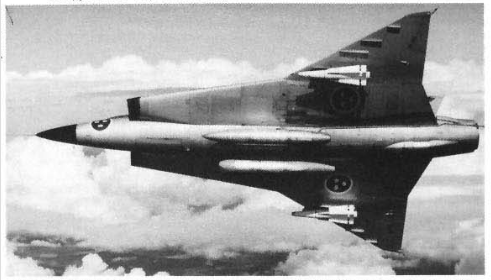
\includegraphics[width=\textwidth]{S35F}
\end{figure}

\LARGE 
Nikolaos Koukis

\vfill
\normalsize \normalfont
Personnummer: 930727T073\\
Date delivered: 2015/02/03\\
Group: D
\end{center}
\end{titlepage}

\newpage
\section{Technical Work}

% Table generated by Excel2LaTeX from sheet 'Sheet1'
\begin{table}[htbp]
  \centering
    \begin{tabular}{p{7cm}|p{7cm}}
    \toprule
    \textbf{Pros}  & \textbf{Cons} \\
    \midrule
    (+)Figure (2) is quite expanatory & (-) What about the dynamic pressure limit? It should have been stated and plotted in the excess thrust graph since the graph include the negative values \\
    (+)Values for $C_{l\beta},C_{lp}$ seem quite reasonable & (-) Equation (2.5) should correspond to $\dot{\phi}$ instead of $\phi$ \\
          & (-) Procedure of calculating $C_{l\beta}$ is not given \\
          & (-) No mathematical proof whatsoever on why the specific equations are used \\
          & (-) Why does the $v-\xi$ curve increases goes up as the $\xi$ values increase? \\
    \bottomrule
    \end{tabular}%
\end{table}%

\section{Content -  structure of report}

% Table generated by Excel2LaTeX from sheet 'Sheet1'
\begin{table}[H]
  \centering
    \begin{tabular}{p{7cm}|p{7cm}}
    \toprule
    \textbf{Pros} & \textbf{Cons} \\
    \midrule
          & (-) High frequency of syntax \\& vocabulary language mistakes \\
          & (-) \quad aircraft's motion $\rightarrow$ motion of the aircraft \\
          & (-) \quad (p.4 par.3) L is defined positive in a clockwise motion from the pilot/fuselage point of view \\
          & (-) \quad (Fig. 7) squar $\rightarrow$ squares \\
          & (-) SEP graph is cropped at 16 km altitude. The maximum altitude is actually higher by a small fraction \\
          & (-) State the goals for optimization in the actual SEP graph (where do we want the aircraft to reach) \\
          & (-) Only 1 optimization case is explained. What about the rest? \\
          & (-) More insight should have been given on the notion of the excess thrust and power. \\
          & (-) Rushed report especially in terms of form. \\
          & (-) Classical introduction "With the jet era starting …" \\
          & (-) Tough for the reader to follow \\
          & (-) Equations (1.1) $\rightarrow$ Mark them as different differential equations \\
    \bottomrule
    \end{tabular}%
\end{table}%


\section{Conclusions}
Minor defects in the structure of the report but apart from that excellent overall 
quality especially for a draft version.




\end{document}
